\section{THESIS}\label{sec:thesis}

\subsection[TYPES OF MASTER'S THESIS]{Types of master's thesis}
\par Start each section from a new page. The second section normally contains a more detailed introduction to the topic. For example, this document might have an introduction to various types for master's thesis.

\subsection[CITING AND REFERENCES]{Citing and references}
\par{Include a cite in the text for all figures, tables, references, and appendices. There are no exceptions for this rule. Use increasing numbering in citing. Appendix 1 acts as an example for an appendix.}

\par{Citing can be as follows: ``In digital imaging contrast enhancement may lead into higher dynamics as shown in Fig. \ref{fig:figimage}.''  If the image is taken from some source, e.g. from a book, the source is mentioned in the caption.  The figure itself comes after the cite in the text, this means that the figure is mentioned in the text before the figure presented. The figure comes after the end of the paragraph. The alignment of the figure and the caption is centered. The caption is always under the figure. The heading of a table is above the table, an example is given in Table \ref{tab:table1}. Table \ref{tab:table1} is an example of a table. The table heading and the table itself are aligned in the center. The texts in the figure caption and in the table heading are closed with a period. The caption and the heading may contain several sentences.}

\begin{figure}[h]
\begin{tabular}{c c}
  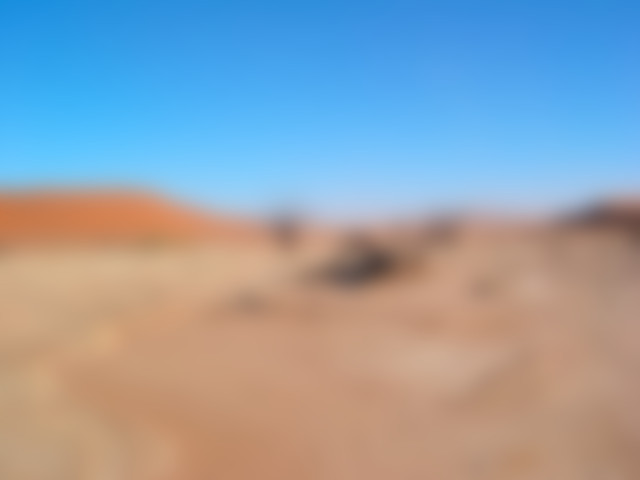
\includegraphics[width=0.45\textwidth]{./figs/image2.jpg} &
  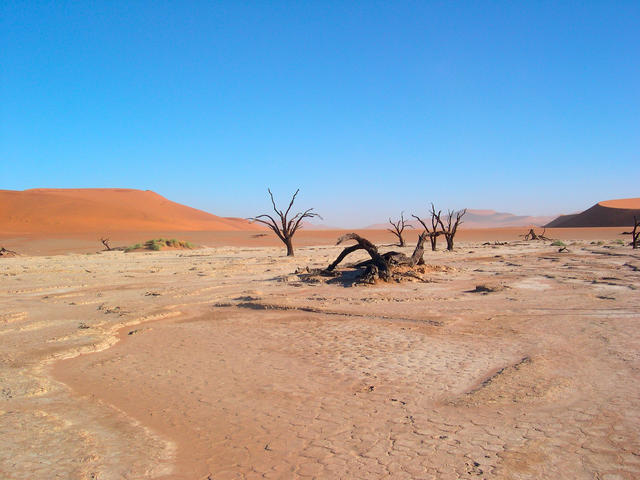
\includegraphics[width=0.45\textwidth]{./figs/image1.jpg}\\
  \hspace{1.2cm}(a) & \hspace{1.2cm}(b) \\
\end{tabular}
\caption[Contrast enhancement.]{Contrast enhancement: a) original image; b) enhanced image \citep{Ahm85}.} \label{fig:figimage}
\end{figure}

\par The figure with the caption and the table with the heading appear as full on one page, do not split them over several pages. For example, Fig. \ref{fig:figimage} and Table \ref{tab:table1} are on one page only. Figures and tables are placed such that there is no extra empty space above or below the image. Normally, figures and tables are placed on top of the page or on the bottom of the page, but they may appear also in the middle. If the figure or the table can not be placed on the same page as the paragraph with the cite then place the figure and the table on the next page. The bottom of the page is filled with the text from the next paragraph.

\begin{table}[h]
  \centering
  \caption[Grading]{Scaling for grading.} \label{tab:table1}
  \begin{tabularx}{0.8\textwidth}{| X | Y | Y | Y | Y |}
  \hline
  Points & 0-10 & 11-20 & 21-30 & 31-40 \\
  \hline
  Grades & 1 & 2 & 3 & 4 \\
  \hline
  \end{tabularx}
\end{table}

\par References are given in the list of references, either in alphabetical order or in citing order. The latter means that the references are listed exactly in the order they are cited in the text. The cites and the corresponding references are numbered as [2] or according to the first author with the year of the publication (K\"{a}lvi\"{a}inen, 2010). If there are several authors, the form for citing is (K\"{a}lvi\"{a}inen, et al., 2008).  All references contain full bibliographic information such that the article can be unambiguously identified. An example for a scientific article [3] and a conference article [4] are here. There is never a cite at the end of a chapter, outside all sentences, i.e. no cite after the dot after the last sentence of a paragraph. The author should always express clearly what comes from a reference and what is produced by the author. 

\par Equations are always numbered and they are part of the text. The presentation is not disconnected because of an equation. Here is an example how to include an equation in the text:

\begin{equation}
   \label{eq:example-equation}
   x=\frac{-b\pm\sqrt{b^2-4ac}}{2a}
\end{equation}

\par Selection operation in genetic algorithms is normally implemented with a so-called roulette table selection where probability PS for the selection of the individual I  is defined as where NP is the size of the population and f is the cost function to be optimized [5].

\par As one can see from Eq. \ref{eq:example-equation} each term and symbol in the equation is introduced and explained and also the reference is given. Normal rules for citing apply also for equations. 

\subsection[EXTENDED EXAMPLE]{Extended Example}
\par The objective of this work is to perform a series of experiments
in rapid dense granular shear flows  to obtain a deeper insight
into corresponding physical and technological facts. Complexity of
flow, deformation dynamics and stability of flow are some
remarkable subjects that deserve precise investigations both
experimentally and theoretically. This work was motivated by the
need of the physics and engineering communities to understand the
basics related to these subjects. As an outcome of this research,
I will show in Chapter \ref{sec:thesis} how the formation of
structures within a granular medium affects the stability of
deformation and flow.

\begin{figure}[h]
  \centering
  \begin{tabular}{c c}
    \hspace{1.2cm}(a) & \hspace{1.2cm}(b) \\
    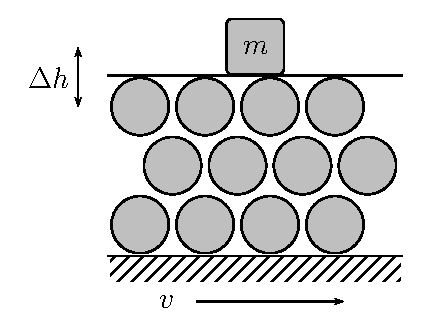
\includegraphics[width=0.4\textwidth]{./figs/comparison2.eps} &
    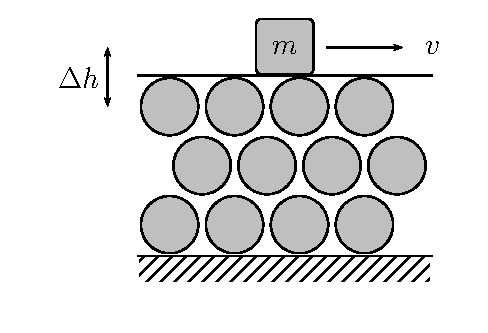
\includegraphics[width=0.46\textwidth]{./figs/comparisonD.eps}\\
    \hspace{1.2cm}(c) & \hspace{1.2cm}(d) \\
    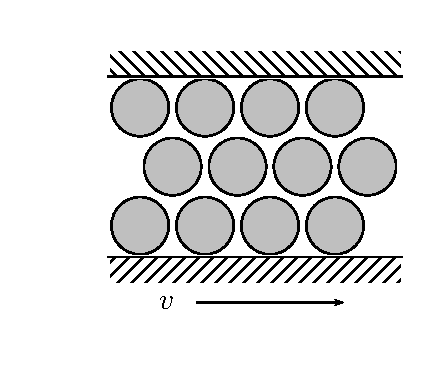
\includegraphics[width=0.4\textwidth]{./figs/comparisonC.eps} &
    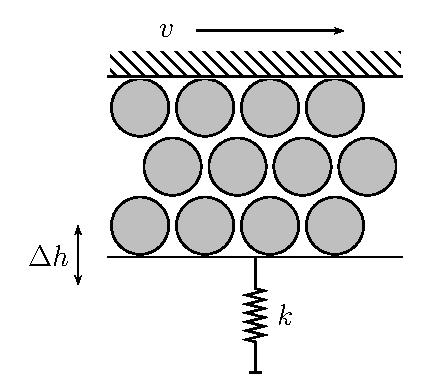
\includegraphics[width=0.4\textwidth]{./figs/comparison3.eps}\\
  \end{tabular}
\caption[Schematics of different types of experimental devices
used to study granular shear flow.]{Schematics of different types of experimental devices
used to study granular shear flow. (a) and (b) represent constant
load devices, where compaction and dilation are allowed. The
difference between (a) and (b) is whether the system is sheared at
the top or from the bottom surface. (c) Constant volume shear
cell. (d) The annular shear cell used in the present study. In the
present experimental device the bottom surface is also allowed to
tilt.} \label{fig:figcomp}
\end{figure}

\clearpage